\documentclass[a4paper,12pt]{article}
\usepackage[brazil]{babel}
\usepackage[utf8]{inputenc}
\usepackage{indentfirst}
\usepackage{amsmath}
\usepackage{graphicx}
\usepackage{animate}
\usepackage{float}
\usepackage[table]{xcolor} % Para colorir as linhas da tabela
\usepackage{array} % Para melhorar a formatação de tabelas
\usepackage[font=footnotesize, labelfont=bf, listformat=empty]{caption}
\usepackage{geometry}
\usepackage{listings}
\usepackage{lastpage}
\usepackage{subcaption}
\usepackage[skins,xparse,breakable]{tcolorbox}
\usepackage{longtable}
\usepackage{minted}
\usepackage{titlesec}
\usepackage{fancyhdr}
\usepackage{setspace}
\usepackage[colorlinks=true, allcolors=black]{hyperref}

% Configurações de margens e espaçamento
\geometry{a4paper, left=3cm, right=2cm, top=3cm, bottom=2cm}
\setlength{\parindent}{1.25cm}
\onehalfspacing

% Configurações de títulos
\titleformat{\section}{\normalfont\large\bfseries}{\thesection}{1em}{}
\titleformat{\subsection}{\normalfont\bfseries}{\thesubsection}{1em}{}
\titleformat{\subsubsection}{\normalfont\itshape}{\thesubsubsection}{1em}{}

% Configurações de listagens
\renewcommand{\listingscaption}{Código}
\newenvironment{code}{\captionsetup{type=listing}}{}

% Configurações de cores
\definecolor{LightSeaGreen}{rgb}{0.1255, 0.6980, 0.6667}
\definecolor{whitesmoke}{rgb}{0.96, 0.96, 0.96}
\definecolor{cinza}{RGB}{160, 160, 160}
\definecolor{cinza_claro}{RGB}{240, 240, 240} % Cinza claro

% Configurações do minted para VHDL
\setminted[VHDL]{
    style=vs,
    linenos=true,
    breaklines=true,
    mathescape=true,
    bgcolor=cinza_claro,
    breakanywhere=true,
}

% Configurações de cabeçalho e rodapé
\pagestyle{fancy}
\fancyhf{}
\fancyhead[L]{\footnotesize{Laboratório de Sistemas Digitais - ENE0040}}
\fancyhead[R]{\footnotesize{2025/1 - Turma 07}}
\fancyfoot[R]{\footnotesize{Página \ \thepage \ de \pageref{LastPage}}}
\fancyfoot[L]{\footnotesize{Relatório do Experimento 2}}

% Adiciona uma linha preta acima do rodapé
\renewcommand{\footrulewidth}{0.4pt} % Espessura da linha
\renewcommand{\footrule}{\vbox to 0pt{\hrule width \textwidth height \footrulewidth \vss}} % Desenha a linha

% Novo Comando para chamar a capa
\newcommand{\capa}{
    \begin{titlepage}
        \begin{center}
            {\large \textbf{ENE0040 - Laboratório de Sistemas Digitais - Turma 07}} \\
            \vspace{3cm}
            {\Huge \textbf{Relatório do Experimento 2}} \\[1em]
            {\large \textbf{Autor:} Henrique Morcelles Salum} \\[0.5em]
            {\large \textbf{Matrícula:} 232003008} \\
            \vfill
            {\Large \textbf{Universidade de Brasília - UnB}} \\[0.75em]
            {\large \textbf{Departamento de Engenharia Elétrica - ENE}} \\
        \end{center}
    \end{titlepage}
}

\begin{document}

\capa

% Sumário
\newpage
\tableofcontents
\newpage

% Introdução
\section{Introdução}

\subsection{Sobre o Experimento}
\paragraph{}
Este experimento é composto por duas tarefas, em ambas, deve-se implementar circuitos lógicos com VHDL e simulá-los por meio do software ModelSim, da Intel. As especificidades de cada tarefa serão exploradas a seguir.

\subsubsection{Somador Completo}
\paragraph{}
Na primeira tarefa, implementa-se um somador completo. As funções booleanas dos sinais de saída $S$ e $C_{out}$ são definidas em função das entradas $A$, $B$ e $C_{in}$ como segue:
\[
S = A \oplus B \oplus C_{in}
\]
\[
C_{out} = A \cdot B + A \cdot C_{in} + B \cdot C_{in}
\]

\subsubsection{Multiplexador 4 para 1}
\paragraph{}
Na segunda tarefa, deve-se implementar um multiplexador de 4 para 1, utilizando dois vetores de entrada: $S$, de dois sinais e $D$, de quatro sinais. A saída é um sinal $Y$ definido da seguinte forma:
\[
Y = D_0 \cdot \overline{S_1} \cdot \overline{S_0} + D_1 \cdot \overline{S_1} \cdot S_0 + D_2 \cdot S_1 \cdot \overline{S_0} + D_3 \cdot S_1 \cdot S_0
\]

\subsection{Introdução Teórica}

\subsubsection{Somador Completo}
\paragraph{}
Antes de definir o somador completo (\textit{Full Adder}), vamos definir o meio somador (\textit{Half Adder}). O meio somador é um circuito lógico combinacional que realiza a soma entre um bit $A$ e um bit $B$. O valor máximo da soma de dois bits $A$ e $B$ é quando $A = 1$ e $B = 1$. O resultado dessa soma é $2$, representado como $10$ em binário. Dessa forma, são necessárias duas saídas para o meio somador: uma para o valor da soma na posição em que estamos e uma para o possível valor da próxima posição, que é igual a 1 quando as duas entradas são 1.

\begin{figure}[H]
    \centering
    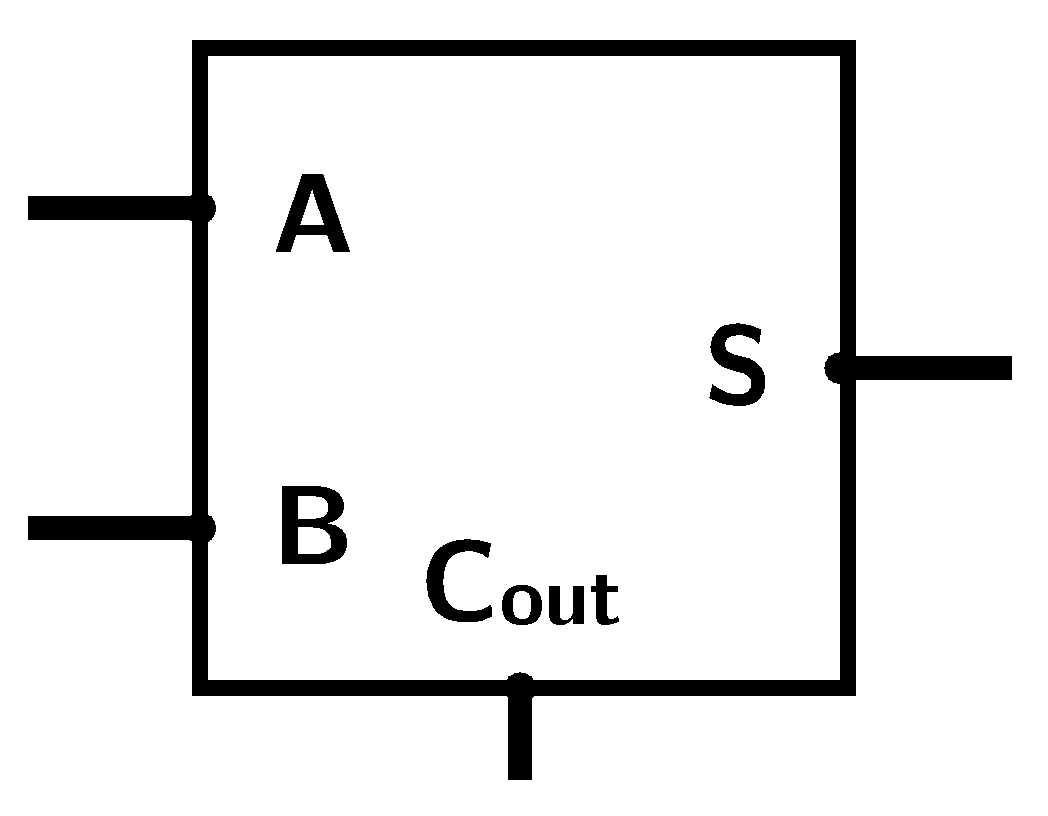
\includegraphics[width=0.3\textwidth]{Imagens/Meio Somador.png}
    \caption{Representação externa do meio somador}
\end{figure}

\paragraph{}
Esse somador, porém, só consegue somar números de um bit. O que fazer, então, se quisermos somar números grandes de vários bits? Para cada posição das representações binárias das entradas, precisamos de um somador para realizar, além da soma entre o bit dessa posição de cada entrada, a soma com o \textit{vai um} da casa anterior - chamaremos de $C_{in}$. O somador que cumpre esses requisitos é chamado somador completo.

\begin{figure}[H]
    \centering
    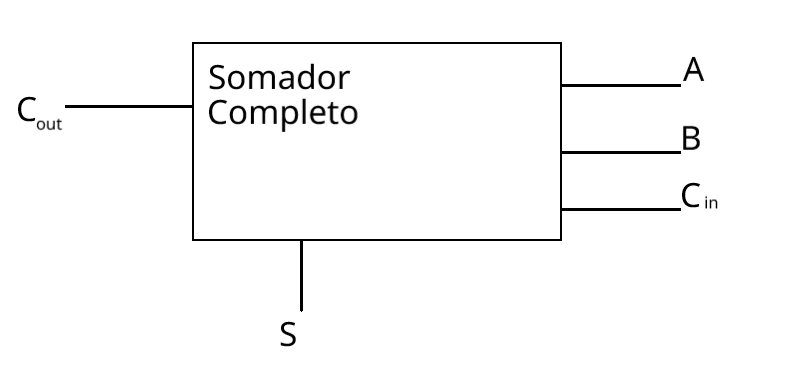
\includegraphics[width=0.35\textwidth]{Imagens/SomadorCompleto.png}
    \caption{Representação externa do somador completo}
    \label{fig:somador_externa}
\end{figure}

\paragraph{}
Note que a representação acima abstrai a lógica que relaciona as saídas do somador às suas entradas. Podemos representar o somador completo pela sua representação interna, que explicita a relação entre entradas e saídas. Essa representação consiste na tradução das equações mostradas na seção ``\textbf{Sobre o Experimento}'' para um esquemático, construído em Logisim.

\begin{figure}[H]
    \centering
    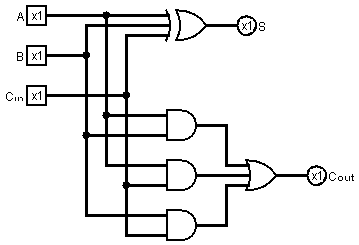
\includegraphics[width=1\linewidth]{Imagens/SomadorCompletoInterno.png}
    \caption{Representação interna do somador completo}
    \label{fig:somador_interna}
\end{figure}

\newpage

\paragraph{}
Para realizar a soma de números grandes, basta encasquetarmos somadores completos. O número de somadores necessários é o número de casas das entradas e a entrada $C_{in}$ de cada somador é a saída $C_{out}$ do somador da posição anterior, com exceção da primeira casa, que tem como entrada $C_{in} = 0$. A tabela-verdade do somador completo é a que segue:

\begin{table}[H]
    \centering
    \begin{tabular}{|c|c|c|c|c|}
        \hline
        \rowcolor{black}
        \multicolumn{3}{|c|}{\textbf{\textcolor{white}{Entradas}}} & \multicolumn{2}{|c|}{\textbf{\textcolor{white}{Saídas}}} \\ \hline
        \rowcolor{black}
        \textcolor{white}{$A$} & \textcolor{white}{$B$} & \textcolor{white}{$C_{in}$} & \textcolor{white}{$C_{out}$} & \textcolor{white}{$S$} \\ \hline
        0 & 0 & 0 & 0 & 0 \\ \hline
        \rowcolor{cinza}
        0 & 0 & 1 & 0 & 1 \\ \hline
        0 & 1 & 0 & 0 & 1 \\ \hline
        \rowcolor{cinza}
        0 & 1 & 1 & 1 & 0 \\ \hline
        1 & 0 & 0 & 0 & 1 \\ \hline
        \rowcolor{cinza}
        1 & 0 & 1 & 1 & 0 \\ \hline
        1 & 1 & 0 & 1 & 0 \\ \hline
        \rowcolor{cinza}
        1 & 1 & 1 & 1 & 1 \\ \hline
    \end{tabular}
    \caption{Tabela-verdade do somador completo}
\end{table}

\subsubsection{Multiplexador 4 para 1}
\paragraph{}
Um multiplexador, também chamado de Mux, é um dispositivo digital que seleciona uma entre várias entradas de dados como saída. Essencialmente, o multiplexador atua como um ``comutador'' controlado por entradas de seleção, determinando qual sinal será encaminhado para a saída. Esse dispositivo é extensivamente usado no projeto de máquinas de estados, pois ele é muito conveniente quando é necessário implementar diferentes lógicas dependendo do estado atual.

\begin{figure}[H]
    \centering
    \includegraphics[width=0.35\textwidth]{Imagens/multiplexador.png}
    \caption{Representação externa do multiplexador 4 x 1}
    \label{fig:Mux_externa}
\end{figure}

\paragraph{}
Para entender esse dispositivo, podemos separar as entradas entre entradas de dados, que são as entradas de informações a serem selecionadas, e as entradas de seleção, que são utilizadas para escolher qual das entradas de dados será enviada para a saída. O número de entradas de seleção pode ser calculado em função do número de entradas de dados pela função: 
\[
f(n) = \lceil \log_2n \rceil
\]
em que $n$ é o número de entradas de dados.

\paragraph{}
Nesse experimento, implementamos, especificamente, um multiplexador 4 para 1, ou seja, um multiplexador com quatro entradas de dados e, consequentemente, $\log_2 4 = 2$ entradas de seleção, além de um sinal de saída. A representação externa do Mux 4x1 já foi apresentada e a interna está a seguir:

\begin{figure}[H]
    \centering
    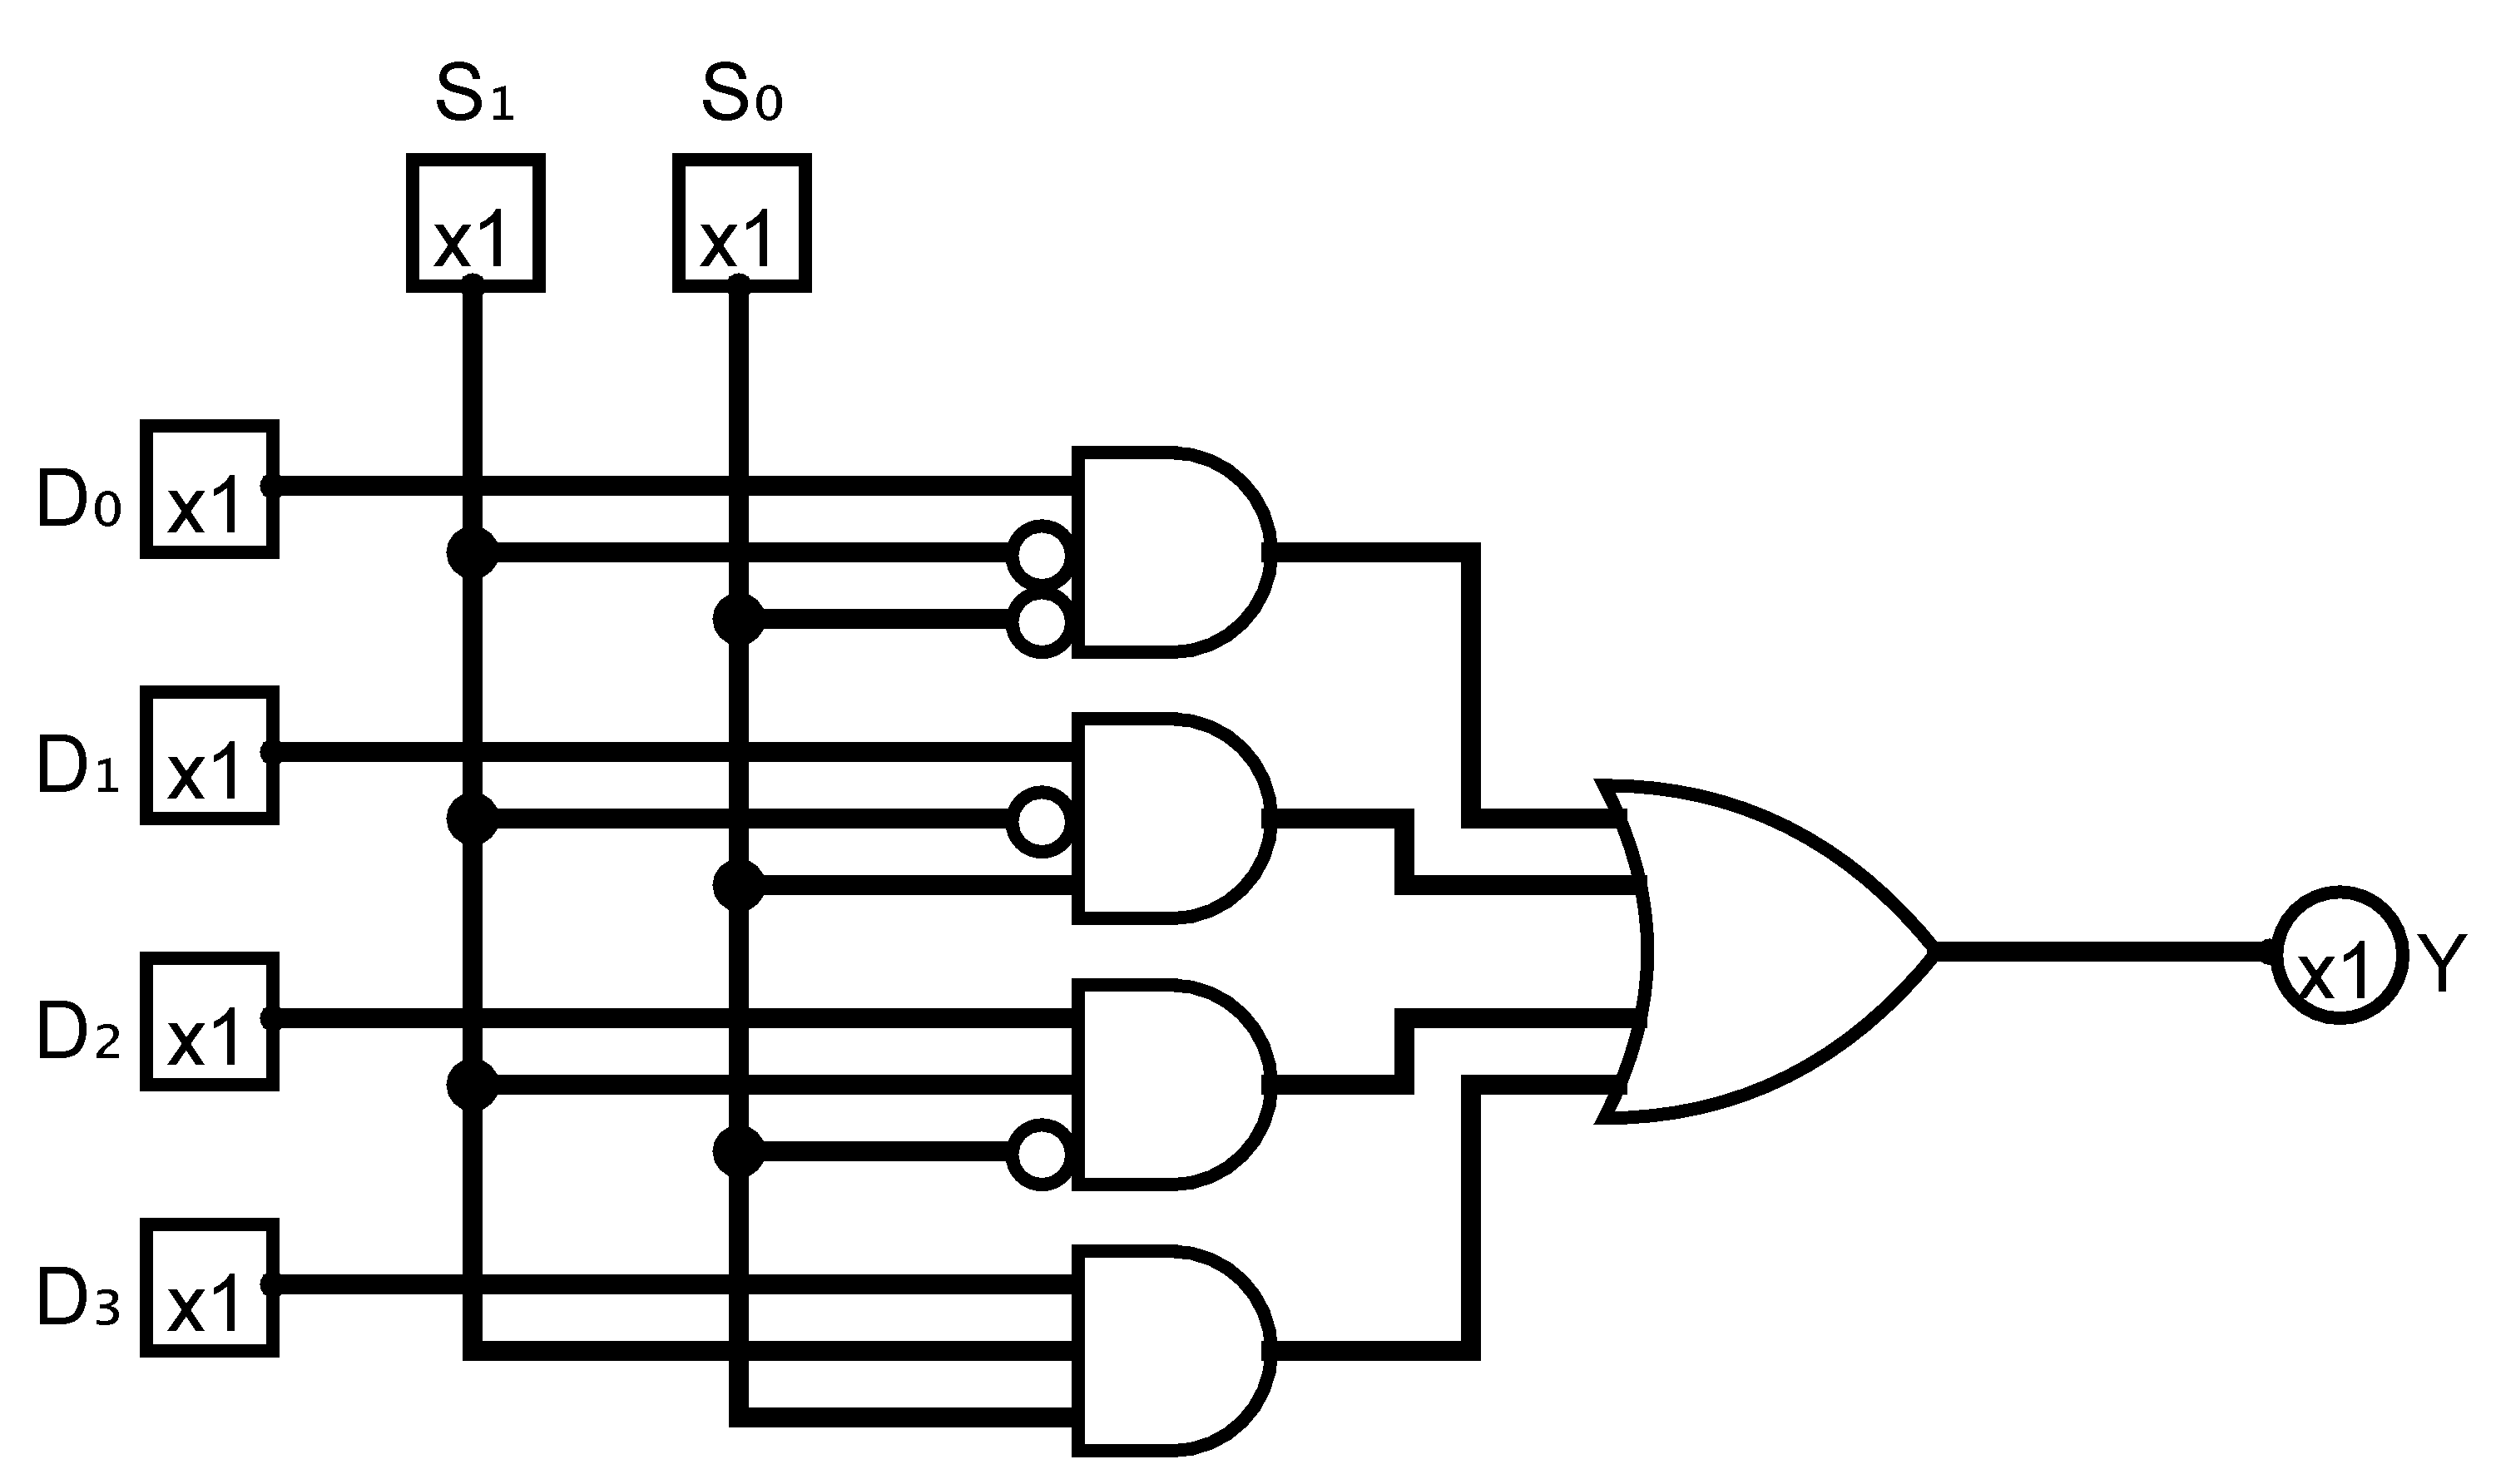
\includegraphics[width=1\linewidth]{Imagens/MultiplexadorInterno.png}
    \caption{Representação interna do multiplexador 4x1}
    \label{fig:Mux_interna}
\end{figure}

\paragraph{}
A tabela-verdade do Mux 4x1, na qual introduzimos a entrada de dados selecionada na saída, ao invés de fazer a tabela para cada variação dessa entrada, é a que segue:

\begin{table}[H]
    \centering
    \begin{tabular}{|c|c|c|}
        \hline
        \rowcolor{black}
        \textcolor{white}{$S_1$} & \textcolor{white}{$S_0$} & \textcolor{white}{Saída} \\ \hline
        0 & 0 & $D_0$ \\ \hline
        \rowcolor{cinza}
        0 & 1 & $D_1$ \\ \hline
        1 & 0 & $D_2$ \\ \hline
        \rowcolor{cinza}
        1 & 1 & $D_3$ \\ \hline
    \end{tabular}
    \caption{Tabela-verdade do multiplexador 4x1}
\end{table}

\newpage

\section{Códigos}
\paragraph{}
Nessa seção, serão apresentados os códigos desenvolvidos, em VHDL, para implementar os sistemas digitais apresentados na introdução. Os códigos referentes ao \textit{design} dos sistemas digitais são apresentados aqui com alguns comentários, os \textit{testbenches}, com bem menos. Os códigos enviados junto a este relatório, porém, estão todos devidamente comentados - aqui, alguns comentários foram suprimidos para melhor apresentação.

\subsection{Somador Completo}
\paragraph{}
Para implementar o somador completo descrito anteriormente, foi necessário desenvolver, em VHDL, o seu \textbf{arquivo de modelo de \textit{hardware}}, composto pela entidade (\textit{entity}), que estabelece a interface do dispositivo, e pela arquitetura (\textit{architecture}), que estabelece a sua lógica interna.

\subsubsection{Descrição de Hardware}
\paragraph{}
O código escrito no arquivo de \textit{design} do somador completo é o que segue:

\begin{code}
\begin{minted}{VHDL}
library IEEE;
use IEEE.std_logic_1164.all;

-- Criação da entidade, que declara entradas e saídas do sistema
entity somadorCompleto is
    port (
        A, B, Cin: in std_logic; -- Entradas
        S, Cout: out std_logic -- Saídas
    );
end somadorCompleto;

-- Criação da arquitetura, que estabelece a lógica entre as entradas e saídas
architecture behavioral of somadorCompleto is
begin
    S <= A xor B xor Cin; -- Lógica da saída S
    Cout <= (A and B) or (A and Cin) or (B and Cin); -- Lógica da saída Cout
end architecture behavioral;
\end{minted}
\caption{Código para implementação do somador completo}
\end{code}

\paragraph{}
A \textit{entity} no código acima é uma representação equivalente à exposta na \textbf{\autoref{fig:somador_externa}}, enquanto a \textit{architecture} é equivalente à representação exposta na \textbf{\autoref{fig:somador_interna}}.

\subsubsection{Testbench}
\paragraph{}
Além do código acima, foi necessário implementar, também em VHDL, um \textit{testbench} para que se pudesse testar o comportamento e a funcionalidade do circuito digital projetado. Com ele, podemos gerar todas as combinações de sinais possíveis e analisar o comportamento do circuito sob cada um desses estímulos. O código para implementar esse \textit{testbench} é o que segue:

\begin{code}
\begin{minted}{VHDL}
library IEEE;
use IEEE.std_logic_1164.all;

-- A entidade do testbench é vazia pois ele nunca será instanciado
entity tb_somadorCompleto is
end tb_somadorCompleto;

architecture testbench of tb_somadorCompleto is
    -- Declaração do componente "somadorCompleto". Pense num componente como uma classe
    component somadorCompleto is
        port (
            A, B, Cin: in std_logic;
            S, Cout: out std_logic
        );
    end component somadorCompleto;
    -- Sinais internos do testbench
    signal A_tb: std_logic := '0';
    signal B_tb: std_logic := '0';
    signal Cin_tb: std_logic := '0';
begin
    -- Inicialização da instância do componente - como se fosse um objeto
    instancia_somador : component somadorCompleto 
        port map (
            A => A_tb,
            B => B_tb,
            Cin => Cin_tb,
            S => open,
            Cout => open
        );
    -- Processo para variar as entradas
    estimulos: process
        variable i: integer := 0;
    begin
        if i /= 0 then
            if i mod 2 = 0 then Cin_tb <= not Cin_tb;
            end if;
            if i mod 4 = 0 then B_tb <= not B_tb;
            end if;
            if i mod 8 = 0 then A_tb <= not A_tb;
            end if;
        end if;

        i := i + 1;
        wait for 6.25 ns;
    end process estimulos;
end architecture testbench;
\end{minted}
\caption{Testbench para o somador completo}
\end{code}

\paragraph{}
No código acima, o somador completo construído é instanciado e utilizado como uma ``caixa-preta''; associamos às suas entradas sinais do \textit{testbench}, o que é equivalente a conectar cabos nas entradas de um dispositivo digital, e, dentro do \textit{process}, fazemos esses sinais oscilarem. Dessa forma, conseguimos testar o dispositivo criado.

\subsection{Multiplexador 4 para 1}
\paragraph{}
Como pôde ser visto, nos códigos relativos ao somador completo, a abordagem foi bastante de baixo nível: não utilizamos abstrações fornecidas pela linguagem VHDL, a função foi implementada diretamente pela equação correspondente e o \textit{testbench} gerou todas as oito possíveis combinações das três entradas. A abordagem para o multiplexador foi diferente, como será observado nos códigos subsequentes.

\subsubsection{Descrição de Hardware}
\paragraph{}
O código desenvolvido em VHDL para implementar a ``caixa-preta'' do multiplexador 4 para 1 é o que segue:

\begin{code}
\begin{minted}{VHDL}
library IEEE;
use IEEE.std_logic_1164.all;

entity Mux4x1 is
    port (
        D: in std_logic_vector(3 downto 0); -- Entradas de dados
        S: in std_logic_vector(1 downto 0); -- Entradas de seleção
        Y: out std_logic -- Saída
    );
end entity Mux4x1;

architecture behavioral of Mux4x1 is
begin
    Y <= D(3) when (S = "11") else -- Lógica da saída
         D(2) when (S = "10") else -- definida em função
         D(1) when (S = "01") else -- das entradas de
         D(0) when (S = "00") else -- seleção
         '-'; -- don't care quando as entradas de seleção são don't cares, weak, alta impedância, etc.
end architecture behavioral;
\end{minted}
\caption{Código para implementação do multiplexador 4x1}
\end{code}

\paragraph{}
Aqui, ao invés de implementar a função pela equação correspondente, foi utilizada uma construção de controle de fluxo `when', em que apenas se definiu o comportamento do circuito para as combinações das entradas de seleção, além de se ter considerado apenas alguns valores - 0 e 1 - para elas, fazendo com que as outras possibilidades - X, Z, H, ... - gerassem saída \textit{don't care} (-). O \textit{testbench} do multiplexador é o que segue.

\paragraph{}
Analogamente ao somador completo, no multiplexador 4 para 1, a entidade (\textit{entity}) é equivalente à representação da \autoref{fig:Mux_externa} e a arquitetura (\textit{architecture}), à da \autoref{fig:Mux_interna}.

\subsubsection{Testbench}
\paragraph{}
O código referente ao \textit{testbench} do multiplexador é o que segue:

\begin{code}
\begin{minted}{VHDL}
library IEEE;
use IEEE.std_logic_1164.all;
use IEEE.numeric_std.all;

entity tb_Mux4x1 is
end entity tb_Mux4x1;

architecture testbench of tb_Mux4x1 is
    component Mux4x1 is
        port (
            D: in std_logic_vector(3 downto 0);
            S: in std_logic_vector(1 downto 0);
            Y: out std_logic
        );
    end component Mux4x1;
    
    signal D_tb: std_logic_vector(3 downto 0) := (others => '1');
    signal S_tb: std_logic_vector(1 downto 0) := (others => '0');
begin
    instancia_Mux4x1: component Mux4x1
        port map (
            D => D_tb,
            S => S_tb,
            Y => open
        );

    -- Processo para variar as entradas de seleção
    estimulos_seletoras: process
        variable s_unsigned: unsigned(1 downto 0);
    begin
        wait for 25 ns;
        s_unsigned := unsigned(S_tb);
        s_unsigned := s_unsigned + 1;
        S_tb <= std_logic_vector(s_unsigned);
    end process estimulos_seletoras;
    
    -- Processo para variar as entradas selecionadas
    variacao_dados: process
        variable i: integer;
    begin
        wait for 12.5 ns;
        -- O índice do elemento do vetor D que é selecionado coincide com o valor do vetor S em inteiro
        i := to_integer(unsigned(S_tb));
        D_tb(i) <= not D_tb(i);
        wait on S_tb;
    end process variacao_dados;
end architecture testbench;
\end{minted}
\caption{Testbench para o multiplexador 4x1}
\end{code}

\paragraph{}
Ao contrário do \textit{testbench} anterior, aqui não são geradas todas as combinações possíveis dos sinais de entrada. Isso se deve à natureza do multiplexador: nele, é irrelevante a variação dos sinais não selecionados em um momento da simulação. Portanto, basta que geremos todas as combinações das entradas de seleção e se verifique se o sinal de saída corresponde à entrada de dados que deve ser selecionada por essa combinação. Para que essa simulação seja mais completa, fez-se com que os sinais de dados selecionados em um momento da simulação oscilassem entre 0 e 1.

% Compilação
\section{Compilação}
\paragraph{}
Após escrever os códigos, é necessário compilá-los pelo ModelSim para que se possa simular os sistemas digitais discutidos. Caso a compilação tenha sucesso, sabemos que não houve erros nos códigos apresentados, mas ainda não podemos afirmar que a lógica para implementar os circuitos está correta; isso será analisado nas próximas seções. A seguir, está a mensagem de compilação dos códigos apresentados acima, sem nenhum erro, como pode ser visto no terminal no canto inferior da figura.

\begin{figure}[H]
    \centering
    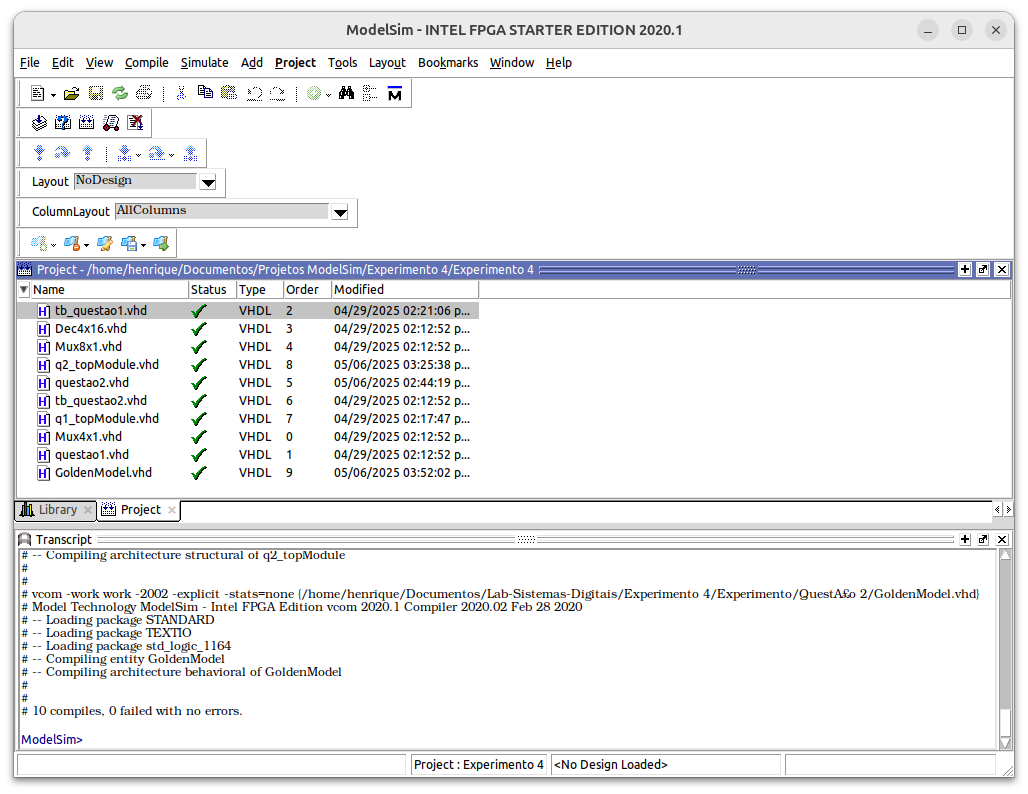
\includegraphics[width=0.75\textwidth]{Imagens/CompileModelSim.png}
    \caption{Compilação de todos os códigos apresentados}
\end{figure}

\section{Simulação}
\paragraph{}
Após compilar com sucesso os códigos apresentados, utilizamos o ModelSim para simular o comportamento dos sistemas descritos por eles. Lá, utilizamos a aba ``Waves'' para analisar o comportamento dos sinais de saída para cada combinação de valores dos sinais de entrada. A forma como as entradas variam segue o que definimos nos \textit{testbenches}, então note que as ondas referentes ao Mux 4x1 não representam todas as combinações das seis entradas. Seguem as imagens das simulações no ModelSim dos sistemas projetados.

\begin{figure}[H]
    \centering
    \begin{tcolorbox}[colframe=darkgray, colback=white, boxrule=0.5pt, arc=1pt, width=0.95\textwidth, center, boxsep=0pt, left=0pt, right=0pt]
    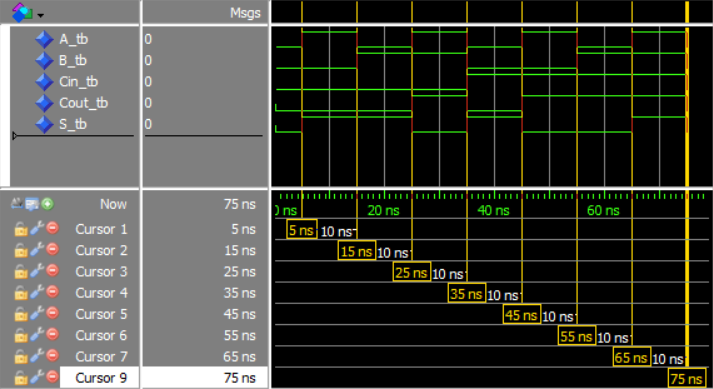
\includegraphics[width=1\textwidth]{Imagens/waves.png}
    \end{tcolorbox}
    \caption{Simulação em forma de onda binária do somador completo}
\end{figure}

\begin{figure}[H]
    \centering
    \begin{tcolorbox}[colframe=darkgray, colback=white, boxrule=0.5pt, arc=1pt, width=0.95\textwidth, center, boxsep=0pt, left=0pt, right=0pt]
    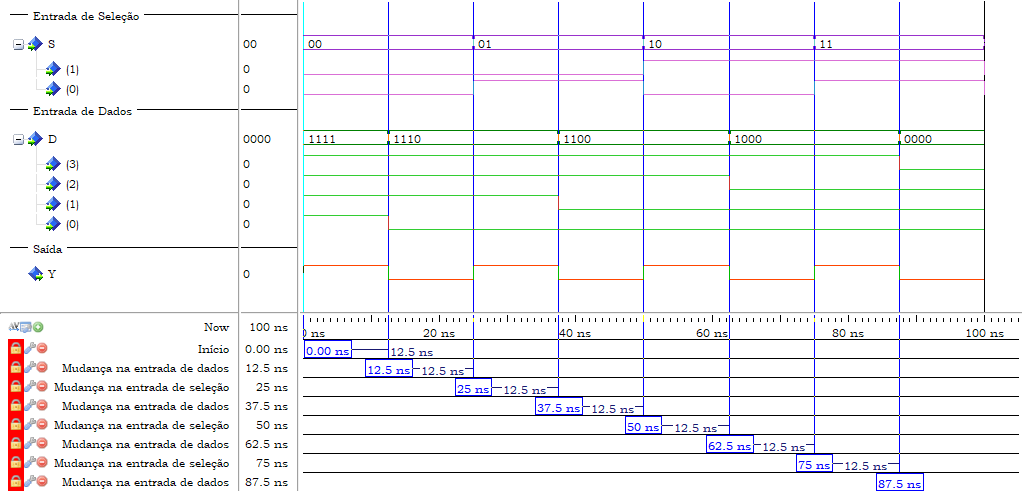
\includegraphics[width=1\textwidth]{Imagens/waves2.png}
    \end{tcolorbox}
    \caption{Simulação em forma de onda binária do multiplexador}
\end{figure}

% Análise
\section{Análise}

\paragraph{}
Para analisar os resultados obtidos, basta olhar para os valores das ondas das entradas e saídas entre cada mudança dos sinais de entrada. Os cursores estão posicionados de forma que, ao selecionar cada um deles, vemos todas as possíveis combinações das entradas e saídas correspondentes na aba à esquerda da tela.

\subsection{Análise do Comportamento do Somador Completo}
\paragraph{}
 Abaixo, exibimos os \textit{prints} que denotam o comportamento dos sinais de saída $S$ e $C_{out}$ para cada combinação dos sinais de entrada $A$, $B$ e $C_{in}$.

\setlength{\fboxsep}{0pt} % Espaçamento entre a borda e a imagem
\begin{figure}[H]
    \centering
    \fcolorbox{cinza}{white}{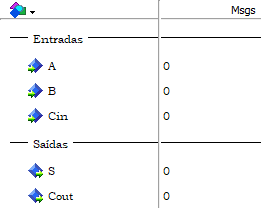
\includegraphics[width=0.3\textwidth]{Imagens/comb1.png}}
    \fcolorbox{cinza}{white}{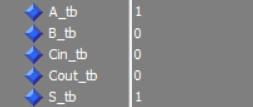
\includegraphics[width=0.3\textwidth]{Imagens/comb2.png}} \\
    \fcolorbox{cinza}{white}{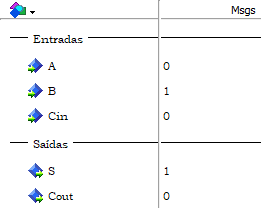
\includegraphics[width=0.3\textwidth]{Imagens/comb3.png}}
    \fcolorbox{cinza}{white}{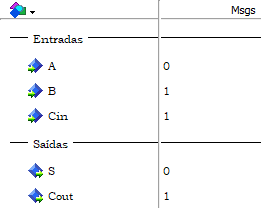
\includegraphics[width=0.3\textwidth]{Imagens/comb4.png}} \\
    \fcolorbox{cinza}{white}{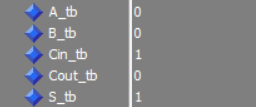
\includegraphics[width=0.3\textwidth]{Imagens/comb5.png}}
    \fcolorbox{cinza}{white}{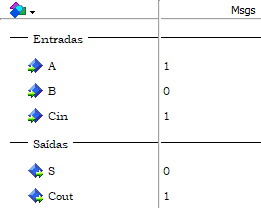
\includegraphics[width=0.3\textwidth]{Imagens/comb6.png}} \\
    \fcolorbox{cinza}{white}{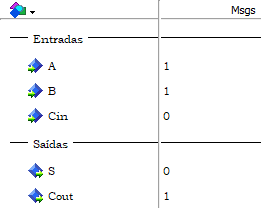
\includegraphics[width=0.3\textwidth]{Imagens/comb7.png}}
    \fcolorbox{cinza}{white}{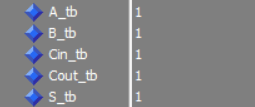
\includegraphics[width=0.3\textwidth]{Imagens/comb8.png}}
    \caption{Todas as combinações possíveis de entradas e as saídas correspondentes do somador completo}
\end{figure}

\paragraph{}
Percebe-se que o comportamento está de acordo com o esperado: a concatenação das saídas $C_{out}$ e $S$ corresponde à soma dos bits de entrada $A$, $B$ e $C_{in}$.

\subsection{Análise do Comportamento do Multiplexador 4 para 1}

\paragraph{}
Para analisar os resultados da simulação do Mux 4x1, observou-se a saída $Y$ para cada combinação da entrada de seleção. Abaixo, estão exibidos os \textit{prints} que mostram o comportamento do circuito simulado pelo ModelSim para cada uma dessas combinações. Perceba que cada linha representa uma combinação das entradas de seleção e, portanto, uma entrada de dados selecionada, enquanto cada coluna representa um possível valor do sinal de entrada de dados selecionado.

\begin{figure}[H]
    \centering
    \includegraphics[width=0.3\textwidth]{Imagens/S=00/11.png}
    \includegraphics[width=0.3\textwidth]{Imagens/S=00/00.png} \\
    \includegraphics[width=0.3\textwidth]{Imagens/S=10/11.png}
    \includegraphics[width=0.3\textwidth]{Imagens/S=10/00.png} \\
    \includegraphics[width=0.3\textwidth]{Imagens/S=01/11.png}
    \includegraphics[width=0.3\textwidth]{Imagens/S=01/00.png}
\end{figure}
\begin{figure}[H]
    \centering
    \includegraphics[width=0.3\textwidth]{Imagens/S=11/11.png}
    \includegraphics[width=0.3\textwidth]{Imagens/S=11/00.png}
\caption{Saídas para todas as combinações das entradas de seleção e de dados selecionadas}
\end{figure}

\noindent Nota-se, em especial, os sinais destacados em cada coluna - sempre o sinal de saída $Y$ e o sinal de entrada selecionado $D_{n}$. É fácil perceber que aquele é igual a este para qualquer combinação das entradas de seleção, ou seja, que a saída é igual ao sinal selecionado, como é, por definição, em um multiplexador.

\section{Conclusão}

\paragraph{}
Nesse experimento, simulou-se, com sucesso, dois dispositivos digitais de suma importância para a eletrônica digital: o somador completo e o multiplexador 4 para 1. No relatório, percebeu-se o sucesso do experimento e pôde-se analisar devidamente os resultados obtidos pelas simulações, por meio das quais foi possível analisar minuciosamente esses dois circuitos e o seu comportamento para cada estímulo possível.

\paragraph{}
Concluindo, não foram observadas discrepâncias entre o comportamento esperado e o observado, podendo-se concluir, portanto, o sucesso do experimento.

\end{document}